\documentclass[border=6pt]{standalone}
\usepackage{tikz}
\usetikzlibrary{arrows.meta,positioning,calc}
\begin{document}
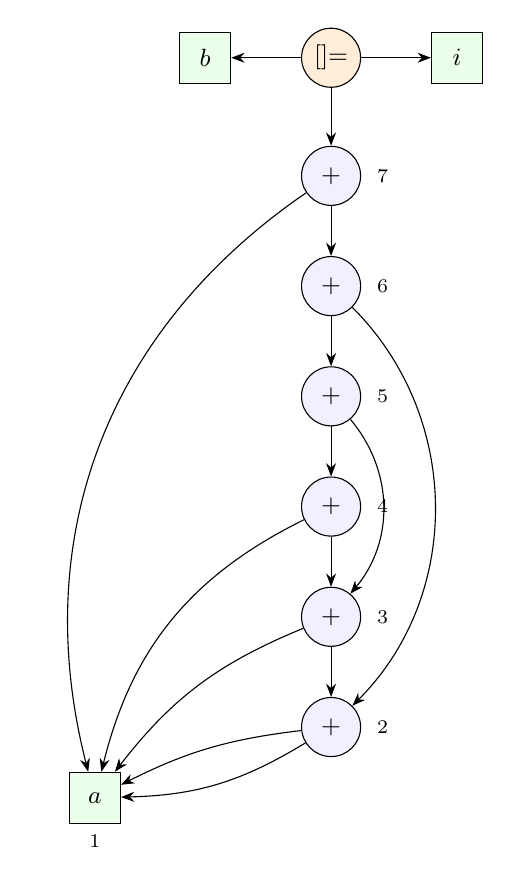
\begin{tikzpicture}[>=Stealth,font=\small,
 op/.style={draw,circle,minimum size=0.75cm,inner sep=0pt,fill=blue!6},
 lf/.style={draw,rectangle,minimum size=0.65cm,inner sep=0pt,fill=green!8},
 nn/.style={font=\scriptsize}]
\node[lf] (a) at (0,0) {$a$}; \node[nn,below=0.02cm of a] {1};
\node[op] (n2) at (3,0.9) {$+$}; \node[nn,right=0.08cm of n2] {2};
\node[op] (n3) at (3,2.3) {$+$}; \node[nn,right=0.08cm of n3] {3};
\node[op] (n4) at (3,3.7) {$+$}; \node[nn,right=0.08cm of n4] {4};
\node[op] (n5) at (3,5.1) {$+$}; \node[nn,right=0.08cm of n5] {5};
\node[op] (n6) at (3,6.5) {$+$}; \node[nn,right=0.08cm of n6] {6};
\node[op] (n7) at (3,7.9) {$+$}; \node[nn,right=0.08cm of n7] {7};
\node[op,fill=orange!15] (as) at (3,9.4) {$[]{=}$};
\node[lf] (b) at (1.4,9.4) {$b$};
\node[lf] (i) at (4.6,9.4) {$i$};
\draw[->] (as)--(b); \draw[->] (as)--(i); \draw[->] (as)--(n7);
\draw[->] (n7)--(n6);
\draw[->] (n6)--(n5);
\draw[->] (n5)--(n4);
\draw[->] (n4)--(n3);
\draw[->] (n3)--(n2);
\draw[->] (n5) to[bend left=40] (n3);
\draw[->] (n6) to[bend left=45] (n2);
\draw[->] (n2) to[bend right=10] (a);
\draw[->] (n2) to[bend left=15] (a);
\draw[->] (n3) to[bend right=15] (a);
\draw[->] (n4) to[bend right=25] (a);
\draw[->] (n7) to[bend right=35] (a);
\end{tikzpicture}
\end{document}
